\documentclass[12pt]{article}
\usepackage[english]{babel}
\usepackage[utf8]{inputenc}
\usepackage{amsmath, amssymb, amsthm}
\usepackage{graphicx}
\usepackage{hyperref}
\usepackage[margin=.75in]{geometry}
\usepackage{xcolor}
\usepackage{tikz}

\setlength{\topmargin}{0pt}
\setlength{\headsep}{0pt}
\textheight = 600pt

\title{Graph Theory \\ Homework 4}
\author{Ben Kallus and Nicholas Adair}
\date{Due Monday, February 15}

\begin{document}
\maketitle

\noindent{\bf 3.2}

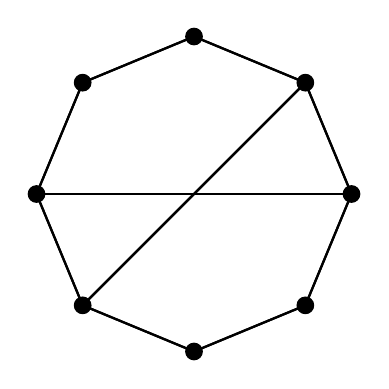
\begin{tikzpicture}
\draw[fill=black] (2.0, 0.0) circle (3pt);
\draw[fill=black] (1.414, 1.414) circle (3pt);
\draw[fill=black] (0.0, 2.0) circle (3pt);
\draw[fill=black] (-1.414, 1.414) circle (3pt);
\draw[fill=black] (-2.0, 0.0) circle (3pt);
\draw[fill=black] (-1.414, -1.414) circle (3pt);
\draw[fill=black] (-0.0, -2.0) circle (3pt);
\draw[fill=black] (1.414, -1.414) circle (3pt);

\draw[thick] (2.0, 0.0) -- (1.414, -1.414);
\draw[thick] (2.0, 0.0) -- (-2.0, 0.0);
\draw[thick] (2.0, 0.0) -- (1.414, 1.414);
\draw[thick] (1.414, 1.414) -- (0.0, 2.0);
\draw[thick] (1.414, 1.414) -- (-1.414, -1.414);
\draw[thick] (1.414, 1.414) -- (2.0, 0.0);
\draw[thick] (0.0, 2.0) -- (-1.414, 1.414);
\draw[thick] (0.0, 2.0) -- (1.414, 1.414);
\draw[thick] (-1.414, 1.414) -- (0.0, 2.0);
\draw[thick] (-1.414, 1.414) -- (-2.0, 0.0);
\draw[thick] (-2.0, 0.0) -- (-1.414, 1.414);
\draw[thick] (-2.0, 0.0) -- (-1.414, -1.414);
\draw[thick] (-2.0, 0.0) -- (2.0, 0.0);
\draw[thick] (-1.414, -1.414) -- (-2.0, 0.0);
\draw[thick] (-1.414, -1.414) -- (-0.0, -2.0);
\draw[thick] (-1.414, -1.414) -- (1.414, 1.414);
\draw[thick] (-0.0, -2.0) -- (1.414, -1.414);
\draw[thick] (-0.0, -2.0) -- (-1.414, -1.414);
\draw[thick] (1.414, -1.414) -- (-0.0, -2.0);
\draw[thick] (1.414, -1.414) -- (2.0, 0.0);
\end{tikzpicture}
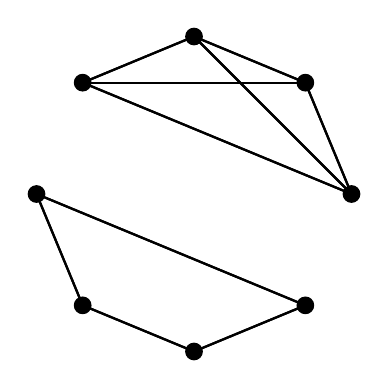
\begin{tikzpicture}
\draw[fill=black] (2.0, 0.0) circle (3pt);
\draw[fill=black] (1.414, 1.414) circle (3pt);
\draw[fill=black] (0.0, 2.0) circle (3pt);
\draw[fill=black] (-1.414, 1.414) circle (3pt);
\draw[fill=black] (-2.0, 0.0) circle (3pt);
\draw[fill=black] (-1.414, -1.414) circle (3pt);
\draw[fill=black] (-0.0, -2.0) circle (3pt);
\draw[fill=black] (1.414, -1.414) circle (3pt);

\draw[thick] (2.0, 0.0) -- (0.0, 2.0);
\draw[thick] (2.0, 0.0) -- (1.414, 1.414);
\draw[thick] (2.0, 0.0) -- (-1.414, 1.414);
\draw[thick] (1.414, 1.414) -- (0.0, 2.0);
\draw[thick] (1.414, 1.414) -- (2.0, 0.0);
\draw[thick] (1.414, 1.414) -- (-1.414, 1.414);
\draw[thick] (0.0, 2.0) -- (2.0, 0.0);
\draw[thick] (0.0, 2.0) -- (1.414, 1.414);
\draw[thick] (0.0, 2.0) -- (-1.414, 1.414);
\draw[thick] (-1.414, 1.414) -- (0.0, 2.0);
\draw[thick] (-1.414, 1.414) -- (2.0, 0.0);
\draw[thick] (-1.414, 1.414) -- (1.414, 1.414);
\draw[thick] (-2.0, 0.0) -- (-1.414, -1.414);
\draw[thick] (-2.0, 0.0) -- (1.414, -1.414);
\draw[thick] (-1.414, -1.414) -- (-0.0, -2.0);
\draw[thick] (-1.414, -1.414) -- (-2.0, 0.0);
\draw[thick] (-0.0, -2.0) -- (-1.414, -1.414);
\draw[thick] (-0.0, -2.0) -- (1.414, -1.414);
\draw[thick] (1.414, -1.414) -- (-0.0, -2.0);
\draw[thick] (1.414, -1.414) -- (-2.0, 0.0);
\end{tikzpicture}
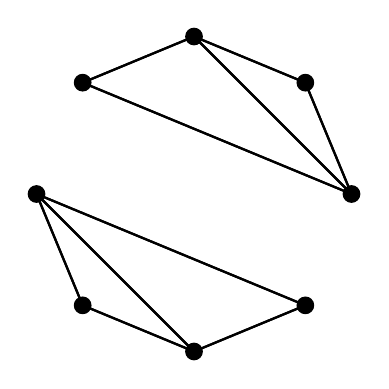
\begin{tikzpicture}
\draw[fill=black] (2.0, 0.0) circle (3pt);
\draw[fill=black] (1.414, 1.414) circle (3pt);
\draw[fill=black] (0.0, 2.0) circle (3pt);
\draw[fill=black] (-1.414, 1.414) circle (3pt);
\draw[fill=black] (-2.0, 0.0) circle (3pt);
\draw[fill=black] (-1.414, -1.414) circle (3pt);
\draw[fill=black] (-0.0, -2.0) circle (3pt);
\draw[fill=black] (1.414, -1.414) circle (3pt);

\draw[thick] (2.0, 0.0) -- (0.0, 2.0);
\draw[thick] (2.0, 0.0) -- (1.414, 1.414);
\draw[thick] (2.0, 0.0) -- (-1.414, 1.414);
\draw[thick] (1.414, 1.414) -- (0.0, 2.0);
\draw[thick] (1.414, 1.414) -- (2.0, 0.0);
\draw[thick] (0.0, 2.0) -- (1.414, 1.414);
\draw[thick] (0.0, 2.0) -- (2.0, 0.0);
\draw[thick] (0.0, 2.0) -- (-1.414, 1.414);
\draw[thick] (-1.414, 1.414) -- (0.0, 2.0);
\draw[thick] (-1.414, 1.414) -- (2.0, 0.0);
\draw[thick] (-2.0, 0.0) -- (-0.0, -2.0);
\draw[thick] (-2.0, 0.0) -- (-1.414, -1.414);
\draw[thick] (-2.0, 0.0) -- (1.414, -1.414);
\draw[thick] (-1.414, -1.414) -- (-2.0, 0.0);
\draw[thick] (-1.414, -1.414) -- (-0.0, -2.0);
\draw[thick] (-0.0, -2.0) -- (-2.0, 0.0);
\draw[thick] (-0.0, -2.0) -- (-1.414, -1.414);
\draw[thick] (-0.0, -2.0) -- (1.414, -1.414);
\draw[thick] (1.414, -1.414) -- (-2.0, 0.0);
\draw[thick] (1.414, -1.414) -- (-0.0, -2.0);
\end{tikzpicture}

\newpage\noindent{\bf 3.4}

Observe that $G_1$ is isomorphic to $G_2$:

\begin{center}
    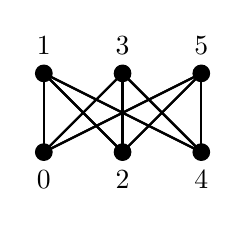
\begin{tikzpicture}
        \draw[fill=black] (0, 0) circle (3pt);
        \node at (0, -0.35) {$0$};
        \draw[fill=black] (0, 1) circle (3pt);
        \node at (0, 1.35) {$1$};
        \draw[fill=black] (1, 1) circle (3pt);
        \node at (1, 1.35) {$3$};
        \draw[fill=black] (2, 1) circle (3pt);
        \node at (2, 1.35) {$5$};
        \draw[fill=black] (1, 0) circle (3pt);
        \node at (1, -0.35) {$2$};
        \draw[fill=black] (2, 0) circle (3pt);
        \node at (2, -0.35) {$4$};

        \draw[thick] (0, 0) -- (0, 1);
        \draw[thick] (0, 0) -- (1, 1);
        \draw[thick] (0, 0) -- (2, 1);
        \draw[thick] (0, 1) -- (0, 0);
        \draw[thick] (0, 1) -- (1, 0);
        \draw[thick] (0, 1) -- (2, 0);
        \draw[thick] (1, 1) -- (0, 0);
        \draw[thick] (1, 1) -- (1, 0);
        \draw[thick] (1, 1) -- (2, 0);
        \draw[thick] (2, 1) -- (0, 0);
        \draw[thick] (2, 1) -- (1, 0);
        \draw[thick] (2, 1) -- (2, 0);
        \draw[thick] (1, 0) -- (0, 1);
        \draw[thick] (1, 0) -- (1, 1);
        \draw[thick] (1, 0) -- (2, 1);
        \draw[thick] (2, 0) -- (0, 1);
        \draw[thick] (2, 0) -- (1, 1);
        \draw[thick] (2, 0) -- (2, 1);
    \end{tikzpicture}
    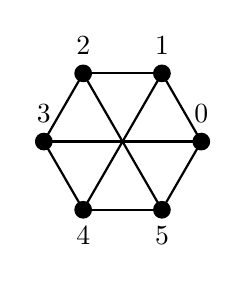
\begin{tikzpicture}
        \draw[fill=black] (1.0, 0.0) circle (3pt);
        \node at (1.0, 0.35) {$0$};
        \draw[fill=black] (0.5, 0.866) circle (3pt);
        \node at (0.5, 1.216) {$1$};
        \draw[fill=black] (-0.5, 0.866) circle (3pt);
        \node at (-0.5, 1.216) {$2$};
        \draw[fill=black] (-1.0, 0.0) circle (3pt);
        \node at (-1.0, 0.35) {$3$};
        \draw[fill=black] (-0.5, -0.866) circle (3pt);
        \node at (-0.5, -1.2) {$4$};
        \draw[fill=black] (0.5, -0.866) circle (3pt);
        \node at (0.5, -1.2) {$5$};

        \draw[thick] (1.0, 0.0) -- (0.5, 0.866);
        \draw[thick] (0.5, 0.866) -- (-0.5, 0.866);
        \draw[thick] (-0.5, 0.866) -- (-1.0, 0.0);
        \draw[thick] (-1.0, 0.0) -- (-0.5, -0.866);
        \draw[thick] (-0.5, -0.866) -- (0.5, -0.866);
        \draw[thick] (0.5, -0.866) -- (1.0, 0.0);
        \draw[thick] (-0.5, 0.866) -- (0.5, -0.866);
        \draw[thick] (0.5, 0.866) -- (-0.5, -0.866);
        \draw[thick] (1.0, 0.0) -- (-1.0, 0.0);
    \end{tikzpicture}
\end{center}

Note that the uppermost three vertices in both $G_3$ and $G_4$ form odd cycles.
Thus, by Theorem 1.12, $G_3$ and $G_4$ are not bipartite.
Thus, by Theorem 3.5, $G_1$ is isomorphic to neither $G_3$ nor $G_4$.
Similarly, $G_2$ is isomorphic to neither $G_3$ nor $G_4$.

Observe that $G_3$ is isomorphic to $G_4$:
\begin{center}
    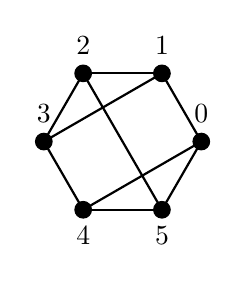
\begin{tikzpicture}
        \draw[fill=black] (1.0, 0.0) circle (3pt);
        \node at (1.0, 0.35) {$0$};
        \draw[fill=black] (0.5, 0.866) circle (3pt);
        \node at (0.5, 1.216) {$1$};
        \draw[fill=black] (-0.5, 0.866) circle (3pt);
        \node at (-0.5, 1.216) {$2$};
        \draw[fill=black] (-1.0, 0.0) circle (3pt);
        \node at (-1.0, 0.35) {$3$};
        \draw[fill=black] (-0.5, -0.866) circle (3pt);
        \node at (-0.5, -1.2) {$4$};
        \draw[fill=black] (0.5, -0.866) circle (3pt);
        \node at (0.5, -1.2) {$5$};

        \draw[thick] (1.0, 0.0) -- (0.5, 0.866);
        \draw[thick] (0.5, 0.866) -- (-0.5, 0.866);
        \draw[thick] (-0.5, 0.866) -- (-1.0, 0.0);
        \draw[thick] (-1.0, 0.0) -- (-0.5, -0.866);
        \draw[thick] (-0.5, -0.866) -- (0.5, -0.866);
        \draw[thick] (0.5, -0.866) -- (1.0, 0.0);
        \draw[thick] (0.5, 0.866) -- (-1.0, 0.0);
        \draw[thick] (1.0, 0.0) -- (-0.5, -0.866);
        \draw[thick] (-0.5, 0.866) -- (0.5, -0.866);
    \end{tikzpicture}
    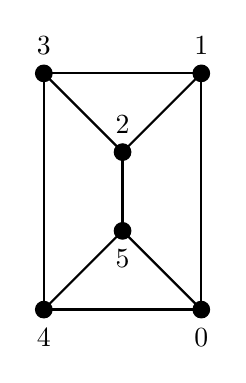
\begin{tikzpicture}
        \draw[fill=black] (0.0, 0.0) circle (3pt);
        \node at (0.0, 0.0-.35) {$4$};
        \draw[fill=black] (0.0, 3.0) circle (3pt);
        \node at (0.0, 3.0+.35) {$3$};
        \draw[fill=black] (2.0, 3.0) circle (3pt);
        \node at (2.0, 3.0+.35) {$1$};
        \draw[fill=black] (2.0, 0.0) circle (3pt);
        \node at (2.0, 0.0-.35) {$0$};
        \draw[fill=black] (1.0, 1.0) circle (3pt);
        \node at (1.0, 1.0-.35) {$5$};
        \draw[fill=black] (1.0, 2.0) circle (3pt);
        \node at (1.0, 2.0+.35) {$2$};

        \draw[thick] (0.0, 0.0) -- (0.0, 3.0);
        \draw[thick] (0.0, 0.0) -- (1.0, 1.0);
        \draw[thick] (0.0, 0.0) -- (2.0, 0.0);
        \draw[thick] (1.0, 1.0) -- (2.0, 0.0);
        \draw[thick] (1.0, 1.0) -- (1.0, 2.0);
        \draw[thick] (0.0, 3.0) -- (2.0, 3.0);
        \draw[thick] (2.0, 3.0) -- (2.0, 0.0);
        \draw[thick] (2.0, 3.0) -- (1.0, 2.0);
        \draw[thick] (0.0, 3.0) -- (1.0, 2.0);
    \end{tikzpicture}
\end{center}

\newpage\noindent{\bf 3.8}

Observe that $G_1$ and $G_2$ are bipartite:
\begin{center}
\includegraphics[scale=.05]{34G1.jpg}
\includegraphics[scale=.05]{34G2.jpg}
\end{center}

Since $G_3$ contains an odd cycle, it is not bipartite by Theorem 1.12.\footnote{An odd cycle of length 5 in $G_3$ can be obtained by choosing a starting vertex, following its ``spoke", then travelling along the outside of the graph until you reach the starting vertex.}

\newpage\noindent{\bf 3.10} Proposition: There does not exist a disconnected self-complementary graph.
\begin{proof}
    Let $G$ be a disconnected graph.
    Then, by Theorem 1.11, $\overline G$ is connected.
    Thus, by Theorem 3.5, $G \not \cong \overline G$.
\end{proof}

\newpage\noindent{\bf 3.12} Proposition: If $G$ and $H$ are self-complementary graphs, and $H$ is of even order $n$ such that $G$ and $H$ have disjoint vertex sets, then the graph obtained from $G \cup H$ by joining each vertex of $G$ to every vertex of degree less than $\frac n2$ in $H$ is self-complementary.
\begin{proof}
    Let $G$ be a self-complementary graph, and let $H$ be a self-complementary graph of even order $n$ such that $G$ and $H$ have disjoint vertex sets.
    Then, there exist isomorphisms $\phi: G \to \overline G, \psi: H \to \overline H$.
    Let $F$ be the graph obtained from $G \cup H$ by joining each vertex of $G$ to every vertex of degree less than $\frac n2$ in $H$.
    Let $\sigma: F \to \overline F$ be defined by $$\sigma(v) = \begin{cases} \phi(v) & v \in V(G), \\ \psi(v) & v \in V(H). \end{cases}$$
    Let $uv \in E(F)$. Consider the following cases:
    
    {\bf Case 1.} $u,v \in V(G)$.
    Then, $\sigma(u)\sigma(v) = \phi(u)\phi(v)$.
    Since $G$ is a subgraph of $F$, $\overline G$ is a subgraph of $\overline F$.
    Thus, since $\phi(u)\phi(v) \in \overline E(G)$, $\phi(u)\phi(v) \in E(\overline F)$.

    {\bf Case 2.} $u,v \in V(H)$.
    By an argument symmetric to case 1, $\phi(u)\phi(v) \in E(\overline F)$.

    {\bf Case 3.} Neither case 1, nor case 2 applies.
    Without loss of generality, let $u \in V(G)$ and let $v \in V(H)$.
    Then, by the definition of $F$, the degree of $v$ in $H$ is less than $\frac n2$.
    Thus, the degree of $\psi(v)$ in $\overline H$ is greater than $\frac n2$.
    Thus,
\end{proof}
\newpage\noindent{\bf 3.16}

\newpage\noindent{\bf 3.17}

{\bf (a)} Yes.

{\bf (b)} No. (Odd cycle)

{\bf (c)} Yes.

\end{document}